%%%%%%%%%%%%%%%%%%%%%%%%%%%%%%%%%%%%%%%%%%%%%%%%%%%%%%%%%%%%%%%%%%%%%%%%%%%%%%%%
\documentclass[12pt]{article}

%%%%%%%%%%%%%%%%%%%%%%%%%%%%%%%%%%%%%%%%%%%%%%%%%%%%%%%%%%%%%%%%%%%%%%%%%%%%%%%%
% META DATA
%%%%%%%%%%%%%%%%%%%%%%%%%%%%%%%%%%%%%%%%%%%%%%%%%%%%%%%%%%%%%%%%%%%%%%%%%%%%%%%%

% Same for each assignment
\newcommand\MYNAME{
	Lolz Consulting Group
	\\
	Quan Dang, Chau Nguyen, Sam Reynolds
}
\newcommand\SHORTNAME{Q. Dang, C. Nguyen, S. Reynolds}
\newcommand\TERM{Fall 2022}
\newcommand\COURSENUMB{STAT 510}
\newcommand\COURSENAME{Basic Statistical Consulting}
\newcommand\SHORTCOURSENAME{Stat. Consulting}

% Different for each assignment
\newcommand\ASSIGNMENTNAME{
	Final Report:
	\\
	Age-dependent Athletic Performance in the
	\\
	Cherry Blossom 10-mile Run Data
}
\newcommand\ASSIGNMENTNAMESHORT{Final Report}
\newcommand\SUBMISSIONDATE{\today}

%%%%%%%%%%%%%%%%%%%%%%%%%%%%%%%%%%%%%%%%%%%%%%%%%%%%%%%%%%%%%%%%%%%%%%%%%%%%%%%%
% PACKAGES
%%%%%%%%%%%%%%%%%%%%%%%%%%%%%%%%%%%%%%%%%%%%%%%%%%%%%%%%%%%%%%%%%%%%%%%%%%%%%%%%

% package for projects with multiple files
\usepackage{subfiles}

% formatting packages
\usepackage[utf8]{inputenc}
\usepackage[margin=3cm]{geometry}
\usepackage{titlesec}	% titles
\usepackage{fancyhdr}	% headers and footers
\usepackage{enumitem}	% better enumerate/itemize environments

% symbol packages
\usepackage{amsmath}
\usepackage{amsthm}
\usepackage{amssymb}
\usepackage{mathtools}

% additional packages
% \usepackage{minted}
% \usepackage{tikz}
% \usepackage{graphicx}
\usepackage{url}
\usepackage{caption}
\usepackage{subcaption}

%%%%%%%%%%%%%%%%%%%%%%%%%%%%%%%%%%%%%%%%%%%%%%%%%%%%%%%%%%%%%%%%%%%%%%%%%%%%%%%%
% FORMATTING
%%%%%%%%%%%%%%%%%%%%%%%%%%%%%%%%%%%%%%%%%%%%%%%%%%%%%%%%%%%%%%%%%%%%%%%%%%%%%%%%

% Page headers
\pagestyle{fancy}
\fancyhf{}
\renewcommand{\headrulewidth}{0pt}
\renewcommand{\footrulewidth}{1pt}
\fancyfoot[C]{\thepage}
\lfoot{\scriptsize \COURSENUMB:~\SHORTCOURSENAME~(\TERM)}
\rfoot{\scriptsize \SHORTNAME:~\ASSIGNMENTNAMESHORT}
\fancypagestyle{plain}{\pagestyle{fancy}} % to get footer on first page

%%%%%%%%%%%%%%%%%%%%%%%%%%%%%%%%%%%%%%%%%%%%%%%%%%%%%%%%%%%%%%%%%%%%%%%%%%%%%%%%
% THEOREM ENVIRONMENTS
%%%%%%%%%%%%%%%%%%%%%%%%%%%%%%%%%%%%%%%%%%%%%%%%%%%%%%%%%%%%%%%%%%%%%%%%%%%%%%%%

%%%%%%%%%%%%%%%%%%%%%%%%%%%%%%%%%%%%%%%%%%%%%%%%%%%%%%%%%%%%%%%%%%%%%%%%%%%%%%%%
% THEOREM ENVIRONMENTS
%%%%%%%%%%%%%%%%%%%%%%%%%%%%%%%%%%%%%%%%%%%%%%%%%%%%%%%%%%%%%%%%%%%%%%%%%%%%%%%%

\usepackage{amsthm}
\usepackage{amsmath}

%%%%%%%%%%%%%%%%%%%%%%%%%%%%%%%%%%%%%%%%%%%%%%%%%%%%%%%%%%%%%%%%%%%%%%%%%%%%%%%%
% FORMATTING
%%%%%%%%%%%%%%%%%%%%%%%%%%%%%%%%%%%%%%%%%%%%%%%%%%%%%%%%%%%%%%%%%%%%%%%%%%%%%%%%

% % bold theorem headers
% \makeatletter
% \newtheoremstyle{bthm}
% 	{3pt}% space before
% 	{3pt}% space after
% 	{\parshape 1 0mm \linewidth}% body font
% 	{0cm}% indent
%  	{\bfseries}% header font
% 	{.}% punctuation
% 	{0.5em}% after theorem header
% 	{}% header specification (empty for default)
% \makeatother
% \theoremstyle{bthm}

%%%%%%%%%%%%%%%%%%%%%%%%%%%%%%%%%%%%%%%%%%%%%%%%%%%%%%%%%%%%%%%%%%%%%%%%%%%%%%%%
% NUMBERING
%%%%%%%%%%%%%%%%%%%%%%%%%%%%%%%%%%%%%%%%%%%%%%%%%%%%%%%%%%%%%%%%%%%%%%%%%%%%%%%%

% determine if the document uses a particular counter
\makeatletter
\newcommand*\ifcounter[1]{%
  \ifcsname c@#1\endcsname
    \expandafter\@firstoftwo
  \else
    \expandafter\@secondoftwo
  \fi
}
\makeatother

% define different numbering scheme for chapters vs. sections
\ifcounter{chapter}{
	% if chapter counter is used, use numbering scheme
	% <chapter> . <section> . x
	\newtheorem{thm}{Theorem}[chapter]
	\numberwithin{thm}{section}
}{
	% if no chapter counter found, use numbering scheme
	% <section> . x
	\newtheorem{thm}{Theorem}[section]
}

%%%%%%%%%%%%%%%%%%%%%%%%%%%%%%%%%%%%%%%%%%%%%%%%%%%%%%%%%%%%%%%%%%%%%%%%%%%%%%%%
% DECLARATIONS
%%%%%%%%%%%%%%%%%%%%%%%%%%%%%%%%%%%%%%%%%%%%%%%%%%%%%%%%%%%%%%%%%%%%%%%%%%%%%%%%

% typical theorem environments
\newtheorem{alg}[thm]{Algorithm}
\newtheorem{cnj}[thm]{Conjecture}
\newtheorem{cor}[thm]{Corollary}
\newtheorem{dfn}[thm]{Definition}
\newtheorem{exm}[thm]{Example}
\newtheorem{lem}[thm]{Lemma}
\newtheorem{prp}[thm]{Proposition}
\newtheorem{rmk}[thm]{Remark}

% less common
\newtheorem{fact}[thm]{Fact}
\newtheorem{goal}[thm]{Goal}
\newtheorem{idea}[thm]{Idea}
\newtheorem{obs}[thm]{Observation}
\newtheorem{q}[thm]{Question}

%%%%%%%%%%%%%%%%%%%%%%%%%%%%%%%%%%%%%%%%%%%%%%%%%%%%%%%%%%%%%%%%%%%%%%%%%%%%%%%%
% MACROS
%%%%%%%%%%%%%%%%%%%%%%%%%%%%%%%%%%%%%%%%%%%%%%%%%%%%%%%%%%%%%%%%%%%%%%%%%%%%%%%%

%%%%%%%%%%%%%%%%%%%%%%%%%%%%%%%%%%%%%%%%%%%%%%%%%%%%%%%%%%%%%%%%%%%%%%%%%%%%%%%%
% Equation Environments
%%%%%%%%%%%%%%%%%%%%%%%%%%%%%%%%%%%%%%%%%%%%%%%%%%%%%%%%%%%%%%%%%%%%%%%%%%%%%%%%
\newcommand\eqn[1]{
	\begin{align*}
		#1
	\end{align*}
}

\newcommand\labeqn[1]{
	\begin{align}
		#1
	\end{align}
}

\newcommand\bracegroup[1]{
	\left\{
	\begin{aligned}
		#1
	\end{aligned}
\right.}

\newcommand\bracketgroup[1]{
	\left[
	\begin{aligned}
		#1
	\end{aligned}
\right.}

%%%%%%%%%%%%%%%%%%%%%%%%%%%%%%%%%%%%%%%%%%%%%%%%%%%%%%%%%%%%%%%%%%%%%%%%%%%%%%%%
% Text Fonts
%%%%%%%%%%%%%%%%%%%%%%%%%%%%%%%%%%%%%%%%%%%%%%%%%%%%%%%%%%%%%%%%%%%%%%%%%%%%%%%%
\newcommand\tbf{\textbf}		% text bold
\newcommand\mono{\texttt}		% fixed width
\newcommand\ul{\underline}		% underlined

%%%%%%%%%%%%%%%%%%%%%%%%%%%%%%%%%%%%%%%%%%%%%%%%%%%%%%%%%%%%%%%%%%%%%%%%%%%%%%%%
% Math Fonts
%%%%%%%%%%%%%%%%%%%%%%%%%%%%%%%%%%%%%%%%%%%%%%%%%%%%%%%%%%%%%%%%%%%%%%%%%%%%%%%%
\renewcommand\bf{\boldsymbol} 	% math bold
\newcommand\bb{\mathbb} 		% blackboard bold
\renewcommand\cal{\mathcal}		% calligraphic
\renewcommand\bar{\overline}	% overline

%%%%%%%%%%%%%%%%%%%%%%%%%%%%%%%%%%%%%%%%%%%%%%%%%%%%%%%%%%%%%%%%%%%%%%%%%%%%%%%%
% Special Letters and Symbols
%%%%%%%%%%%%%%%%%%%%%%%%%%%%%%%%%%%%%%%%%%%%%%%%%%%%%%%%%%%%%%%%%%%%%%%%%%%%%%%%
\newcommand{\ii}{\mathfrak{i}} 	% complex i
\newcommand{\eps}{\varepsilon}	% curvy epsilon
\newcommand{\phii}{\varphi} 	% curvy phi

%%%%%%%%%%%%%%%%%%%%%%%%%%%%%%%%%%%%%%%%%%%%%%%%%%%%%%%%%%%%%%%%%%%%%%%%%%%%%%%%
% Brackets, Braces, and Bars
%%%%%%%%%%%%%%%%%%%%%%%%%%%%%%%%%%%%%%%%%%%%%%%%%%%%%%%%%%%%%%%%%%%%%%%%%%%%%%%%
\DeclarePairedDelimiter{\paren}{ ( }{ ) }			% parentheses
\DeclarePairedDelimiter{\bracket}{ [ }{ ] }			% square brackets
\DeclarePairedDelimiter{\curly}{ \{ }{ \} }			% curly braces
\DeclarePairedDelimiter{\abs}{|}{|}					% absolute value
\DeclarePairedDelimiter{\norm}{\|}{\|}				% norm
\DeclarePairedDelimiter{\ip}{\langle}{\rangle}		% inner product
\DeclarePairedDelimiter{\ceil}{\lceil}{\rceil} 		% ceiling
\DeclarePairedDelimiter{\floor}{\lfloor}{\rfloor} 	% floor

%%%%%%%%%%%%%%%%%%%%%%%%%%%%%%%%%%%%%%%%%%%%%%%%%%%%%%%%%%%%%%%%%%%%%%%%%%%%%%%%
% Sets
%%%%%%%%%%%%%%%%%%%%%%%%%%%%%%%%%%%%%%%%%%%%%%%%%%%%%%%%%%%%%%%%%%%%%%%%%%%%%%%%
\newcommand{\nada}{\varnothing} % empty set
\newcommand{\C}{\mathbb{C}}
\newcommand{\F}{\mathbb{F}}
\newcommand{\N}{\mathbb{N}}
\newcommand{\Q}{\mathbb{Q}}
\newcommand{\R}{\mathbb{R}}
\newcommand{\Z}{\mathbb{Z}}

%%%%%%%%%%%%%%%%%%%%%%%%%%%%%%%%%%%%%%%%%%%%%%%%%%%%%%%%%%%%%%%%%%%%%%%%%%%%%%%%
% Algebra
%%%%%%%%%%%%%%%%%%%%%%%%%%%%%%%%%%%%%%%%%%%%%%%%%%%%%%%%%%%%%%%%%%%%%%%%%%%%%%%%
\newcommand\inv{^{-1}} % inverse

%%%%%%%%%%%%%%%%%%%%%%%%%%%%%%%%%%%%%%%%%%%%%%%%%%%%%%%%%%%%%%%%%%%%%%%%%%%%%%%%
% Matrices
%%%%%%%%%%%%%%%%%%%%%%%%%%%%%%%%%%%%%%%%%%%%%%%%%%%%%%%%%%%%%%%%%%%%%%%%%%%%%%%%
\newcommand{\pmat}[1]{\begin{pmatrix}#1\end{pmatrix}} % soft
\newcommand{\bmat}[1]{\begin{bmatrix}#1\end{bmatrix}} % hard

%%%%%%%%%%%%%%%%%%%%%%%%%%%%%%%%%%%%%%%%%%%%%%%%%%%%%%%%%%%%%%%%%%%%%%%%%%%%%%%%
% Linear Algebra
%%%%%%%%%%%%%%%%%%%%%%%%%%%%%%%%%%%%%%%%%%%%%%%%%%%%%%%%%%%%%%%%%%%%%%%%%%%%%%%%

\renewcommand\t{^\intercal} 			% transpose
\newcommand\spn{\operatorname{span}} 	% span
\newcommand\range{\operatorname{range}}	% range
\newcommand\nul{\operatorname{null}} 	% null space
\newcommand\rank{\operatorname{rank}} 	% rank
\newcommand\trace{\operatorname{tr}} 	% trace
\newcommand\diag{\operatorname{diag}}	% diagonal

%%%%%%%%%%%%%%%%%%%%%%%%%%%%%%%%%%%%%%%%%%%%%%%%%%%%%%%%%%%%%%%%%%%%%%%%%%%%%%%%
% Calculus
%%%%%%%%%%%%%%%%%%%%%%%%%%%%%%%%%%%%%%%%%%%%%%%%%%%%%%%%%%%%%%%%%%%%%%%%%%%%%%%%

\renewcommand\div{\text{div}\;}
\newcommand\curl{\text{curl}\;}

% Additional macros

\newcommand{\foo}{your wish is my command}

%%%%%%%%%%%%%%%%%%%%%%%%%%%%%%%%%%%%%%%%%%%%%%%%%%%%%%%%%%%%%%%%%%%%%%%%%%%%%%%%
 % FRONT MATTER
%%%%%%%%%%%%%%%%%%%%%%%%%%%%%%%%%%%%%%%%%%%%%%%%%%%%%%%%%%%%%%%%%%%%%%%%%%%%%%%%

\title{\large
	\ASSIGNMENTNAME
	\\~\\
	\COURSENUMB:
	\\
	\COURSENAME
}
\author{\MYNAME}
\date{\SUBMISSIONDATE}

%%%%%%%%%%%%%%%%%%%%%%%%%%%%%%%%%%%%%%%%%%%%%%%%%%%%%%%%%%%%%%%%%%%%%%%%%%%%%%%%
% BODY
%%%%%%%%%%%%%%%%%%%%%%%%%%%%%%%%%%%%%%%%%%%%%%%%%%%%%%%%%%%%%%%%%%%%%%%%%%%%%%%%

\begin{document}
\maketitle

%%%%%%%%%%%%%%%%%%%%%%%%%%%%%%%%%%%%%%%%%%%%%%%%%%%%%%%%%%%%%%%%%%%%%%%%%%%%%%%%
% EXERCISES
%%%%%%%%%%%%%%%%%%%%%%%%%%%%%%%%%%%%%%%%%%%%%%%%%%%%%%%%%%%%%%%%%%%%%%%%%%%%%%%%

\section*{Executive Summary}

From our analysis, we found that age does have a significant factor in your physical ability. Evidence suggests that there is a peak age at which physical ability is best, occurring around the age of 26 for both men and women. Furthermore, aging affects differently between genders, and among runners at different levels. Overall, from our findings, we can conclude that as people age, their physical ability worsens.



\section*{Introduction}

The overall goal of this project is to determine how age relates to physical ability, specifically performance in a marathon. To answer this question, we also need to see what the statistically “average” runner was like. This included finding out how old the average runner was, what the average time to complete the race would be, as well as how many participants came back to run again in multiple races. Moreover, we wanted to look at the performance of people who have participated multiple times; did they improve as they aged, or did they stay the same/get slower? Aiming to answer this question, we analyzed the data collected from the Cherry Blossom 10 Mile Run to draw correlations between a runner’s age and how fast they ran the race. Finally, using all of the data we collected, we sought to determine the age at which runners were the most physically fit. In our case, this would be the age where runners were the fastest. One hypothesis that we wanted to confirm was that there is a trend of physical ability getting worse past a certain age. We also look into the declining rate of performance among different groups of runners to see if slower runners slow down at a lower or higher rate compared to faster ones.


\section*{Background}

This study utilizes information from runners of the Cherry Blossom 10 Mile Run, which is an annual marathon held in Washington D.C. each Spring, typically at the start of April. The race is often used as training for those who are participating in other footraces, so we can expect many of the runners to be more active than the average person. The race began in 1973, and race participation grew steadily until 2020, when race participation drastically fell due to the Covid-19 pandemic. For this reason, we opted to examine only data of 47 years from 1973 through 2019. We obtained the data on race participants from the Cherry Blossom Ten Mile Run website via web scraping.


\section*{Data}

The data we used was collected through the Cherry Blossom 10 Mile Run database. The most important pieces of information that we kept track of include: the year of the race, the name of the racer, their gender, their time and pace of the race, where they came from (hometown), and what position they finished in. For our analysis, we decided to convert the time to minutes, and also convert the pace to minutes per mile. Once we had collected the data from the database, we were left with around 340 thousand entries to work with. However, one problem is that for the first 5 years, many of the recorded runs had information that we had to exclude due to unclarity. These ranged from hometowns to division and age. Age was particularly important because it is the main explaining factor of physical performance that this study focuses on. Because of this, we may see some inconsistencies, particularly in the earlier years, as there isn’t as much data as later on when more people started participating. After cleaning the data of missing key values, we were left with around 320 thousand entries. Using the data we extracted and cleaned, we were able to create a list of unique runners using a combination of the runner’s name, birth year (the year of the race subtracted by the age of the participant), gender, and hometown. By doing so, we are able to identify some of the runners as participating in multiple races, and thereby follow their performance as they age. Although there is a limit of 140 minutes for runners to complete the race, some records broke this limit. We decide to keep those observations since they might reflect the actual racing time of people rather than censoring and systematically biasing the data.


\section*{Methods}

In this study, we use descriptive statistics and linear regression to uncover
the relationship between aging and physical performance (proxied by race
running time).
From the original dataset, we managed to track runners that participated in
multiple races.
Therefore, we have two types of regression analysis: cross-sectional and panel
(longitudinal) analysis.
The cross-sectional analysis uses the cleaned version of the original dataset
where each record of runners is one secluded data point and the chronological
order of data is ignored---this means that the same person who participated
in two different races will have two records that are treated as if they
belong to two different people. Meanwhile, the panel (longitudinal) analysis
is based on a data-rich subset of the original data, where records of runners
are identified if they belong to the same person, which adds a time
dimension to the information and helps reveal the temporal variation
of individuals.

The panel analysis is considered superior to the other given concerns about
confounding factors related to both age and physical performance.
For example, new trends of healthier lifestyles in the U.S. population or
medical advances might improve people's health and physical performance in
general, and these trends that can affect the mass population simultaneously
are time-related, thus, age-related.
In such a case, over a certain period of time, the running performance is
not worsening (increasing running time) as much as it would in the
counterfactual scenario where those trends did not emerge.
In other words, the effect of aging on physical fitness will not be truly
reflected by the data and will be underestimated.
Panel regression introduces year-dummy variables to control for those
confounding factors that are related to both the predictors
(i.e. age in our study) and the response (i.e. physical performance or
running time in our study), which helps bring the estimation closer to
the true relationship between aging and physical fitness.


However, these dummy variables are unable to remove those confounding
factors related to both age and running time but do not affect everyone
at the same point in time.
If aging leads to better choices of diets and/or physical activities as
people become wiser when it comes to health, information on diets and
physical activities should be included for control to help single out the
pure effect of aging.

\section*{Results}

\subsubsection*{Overview from descriptive analysis}


\begin{figure}[ht]
	\centering
	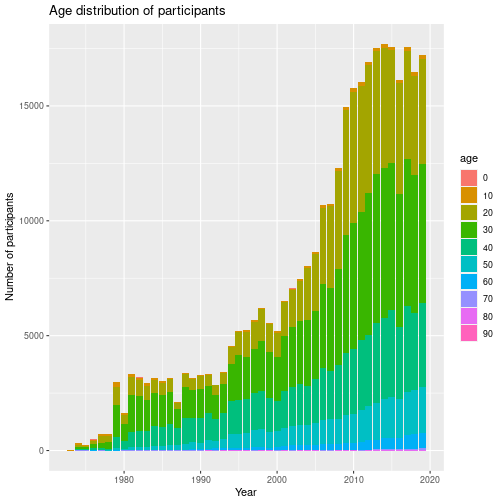
\includegraphics[width = 0.8\textwidth]
	{../figure/descriptive_stat-1.png}
	\caption{
		The age distribution of participants for each year.
		Colors represent age group.
	}
	\label{age-dist}
\end{figure}

% \begin{figure}
% 	\centering
% 	\begin{subfigure}{0.49\textwidth}
% 		\includegraphics[width = \textwidth]
% 		{../figure/descriptive_stat-1.png}
% 		\caption{}
% 		\label{age-dist-1}
% 	\end{subfigure}
% 	\hfill
% 	\begin{subfigure}{0.49\textwidth}
% 		\includegraphics[width = \textwidth]
% 		{../figure/descriptive_stat-2.png}
% 		\caption{}
% 		\label{age-dist-2}
% 	\end{subfigure}
% 	\caption{
% 		(a) The age distribution of participants for each year.
% 		Colors represent age group.
% 		(b) The age proportion of participants for each year.
% 	}
% 	\label{age-dist}
% \end{figure}

\begin{figure}[ht]
	\centering
	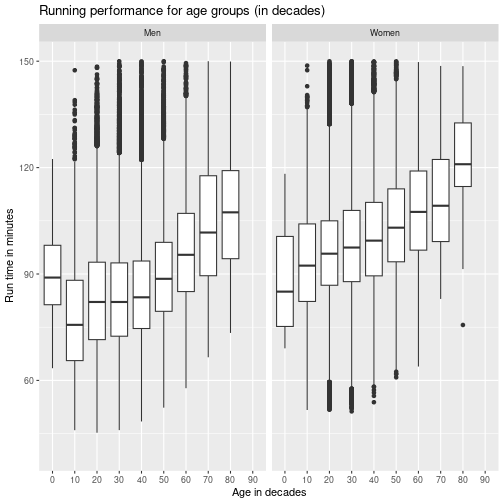
\includegraphics[width = 0.75\textwidth]
	{../figure/boxplot_runtime_age-1.png}
	\caption{
		Time for participants to complete the race for each age group.
		Dots denote outliers. Half of participants in a given age group
		lie inside the boxed interval.
	}
	\label{box-plot}
\end{figure}

The majority of the runners are from 20 to 50 years old.
More people are participating in the race over the years.
The number of women completing the marathon surpassed that of men since
around 2005 and the trend continues until 2019.

There used to be a higher proportion of under-10-year-old marathon
runners before 1990 when the race was not as popular as it is nowadays.
As the race gets more popular, it attracts more people in their 20s and 30s
who have outnumbered those of other age groups.

Using cross-sectional data, the general trend is that performance worsens as
people age. The median runner's performance is increasing with older age groups.
By looking at the outliers, the best performers are in their 20s and 30s.
By each age group, men outperform women.
The fastest male runners' speed is not far higher from that of the majority
while the best female runners are exceptionally better than their majority
peers (there are more lower-bound outliers in women's plot).

\subsubsection*{The general effect of aging on
	men's and women's racing performance}

\begin{figure}[ht]
	\centering
	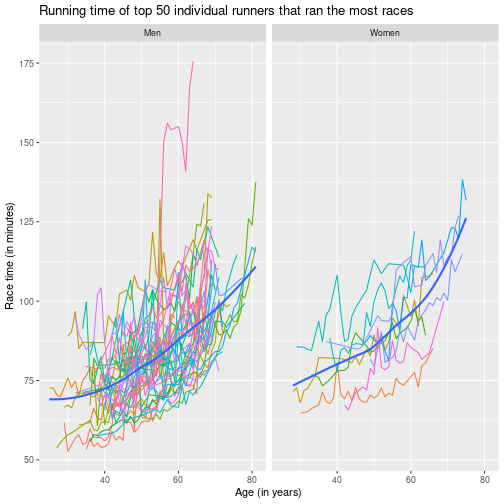
\includegraphics[width = 0.75\textwidth]
	{../figure/overview_tracked_runners-4.png}
	\caption{
		Top 50 participants who participated in the most races.
		As participants age, their time to complete the race
		tends to increase.
	}
	\label{tracked-runners-smooth}
\end{figure}

Using the tracked runners dataset, after averaging and smoothing multiple
runners' performance, two possible models for this data are linear and
quadratic regression.

After fitting two models, our statistical criterion suggests that linear
regression should be preferred.
Residual diagnostics also suggest that log-transformed running time should
be the response variable.
And the result of time-fixed effect model regression is:
% Wow don't the equation editor it is cursed
\begin{align*}
	\log(\text{Runningtime})
	= b_0 &+ 0.005114592 \cdot \text{age}
	\\&
	+ 0.235572473 \cdot \text{gender}
	\\&
	- 0.002457131 \cdot \text{age:gender}
\end{align*}


All estimate coefficients are statistically significant at 1\% level.
We can be 99\% confident that:
\begin{enumerate}[label=(\roman*)]
	\item for men, getting one year older is associated with a 0.5\%
		increase in running time, which is translated into 5.2\% after a decade;
	\item for women, one year older is associated with 0.3\% increase in
		running time $\sim$ 2.7\% after a decade;
	\item female runners' declining rate per year is 0.2\% less than that of
		men; and
	\item on average, women are slower than men by 26.6\%.
\end{enumerate}

\subsubsection*{Declining performance rate for different types of runners}

\begin{figure}
	\centering
	\begin{subfigure}[]{0.49\textwidth}
		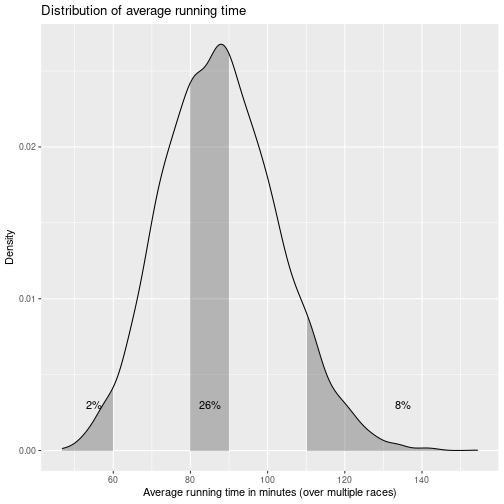
\includegraphics[width = \textwidth]
		{../figure/elite_vs_nonelite_gr0-2.png}
		\caption{}
		\label{type123-dist}
	\end{subfigure}
	\begin{subfigure}[]{0.49\textwidth}
		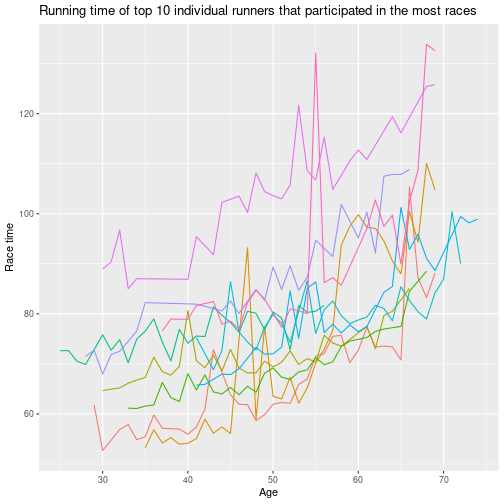
\includegraphics[width = \textwidth]
		{../figure/overview_tracked_runners-2.png}
		\caption{}
		\label{top-10-tracked}
	\end{subfigure}
	\caption{
		(a) The top 20\%, middle 20\%, and bottom 20\% of
			tracked runners were considered type 1, type 2, and
			type 3, respectively.
		(b) The time to complete the race increases for the
			tracked runners as they aged.
	}
	\label{type123}
\end{figure}

% \begin{figure}
% 	\centering
% 	\includegraphics[width = 0.49\textwidth]
% 	{../figure/elite_vs_nonelite_gr0-2.png}
% 	\label{type123-dist}
% 	\caption{I need a caption}
% \end{figure}

% \begin{figure}
% 	\centering
% 	\includegraphics[width = 0.49\textwidth]
% 	{../figure/overview_tracked_runners-2.png}
% 	\label{top-10-tracked}
% 	\caption{I need a caption}
% \end{figure}

To test the declining rate of different types of runners,
we separated runners into five quintiles and selected three different
groups depending on their average run times between all of the years they
raced; see Figure \ref{type123-dist}.
Type 1 are the fastest 20\% of runners, type 2 are the middle 20\% and
type 3 are the slowest 20\%.
We discard the runners in-between these three groups to draw a clearer
distinction between them.
From this, we found that the fastest runners completed the race faster
than 72 minutes for men and 85 minutes for women.
The median runners were between 79-86 minutes for men and 92-99 minutes
for women.
And lastly, the slowest runners took at least 94 minutes for men and
107 minutes for women to complete.

\begin{figure}[ht]
	\centering
	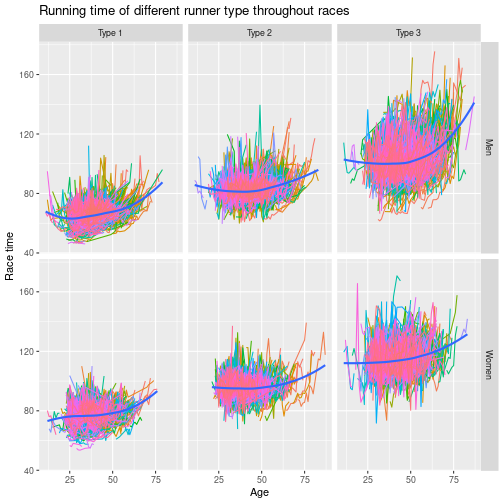
\includegraphics[width = 0.8\textwidth]
	{../figure/run_type2_gr-1.png}
	\caption{
		The time to complete the race for tracked runners of
		type 1,2,3 from left to right. Top row is men,
		bottom row is women.
		The trend curve suggests that runners are most physically
		fit in their mid 20s.
	}
	\label{type123-trend}
\end{figure}

Next, we compared the trends between each type;
see Figure \ref{type123-trend}.
From this, we saw there was a relationship between runners' speed and how
much they declined in performance each year.
Type 3 runners on average declined in performance the most at a rate
of approximately 3.1 minutes per decade for men and 1.8 minutes per
decade for women.
Meanwhile, type 2 runners declined the least for both sexes at about
1.3 minutes per decade for men and 0.7 minutes per decade for women.
Finally, type 1 runners were in between type 3 and 2 at an average of
around 2 minutes per decade for men and 1.1 minutes per decade for women.

From this, we hypothesized that slow runners in type 3 were usually
composed of more older runners, so age will have a much more dramatic
impact on their time as they age.
Comparatively, the faster runners in type 1 may have been composed of
more people who specifically train for races and marathons,
so they may have a higher chance of burning out or sustaining injuries
as they run, thus having a decent declining rate compared to the
average person.
As for type 2, they are most likely made of average marathon
participants who %mainly keep their performance from year to year.
manage to sustain their performance throughout the years
\subsubsection*{Age of peak performance}

\begin{figure}
	\centering
	\begin{subfigure}{0.49\textwidth}
		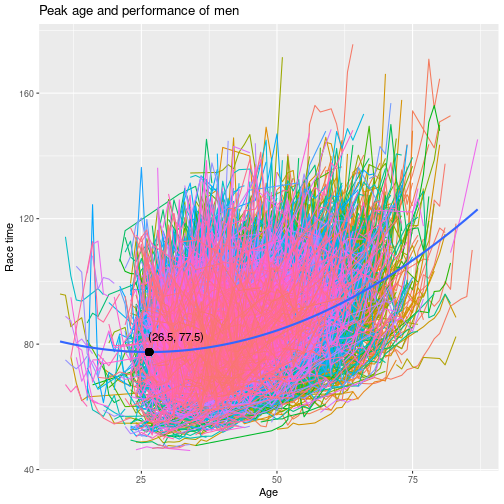
\includegraphics[width = \textwidth]
		{../figure/peak_plot2-1.png}
		\caption{}
		\label{peak-men}
	\end{subfigure}
	\hfill
	\begin{subfigure}{0.49\textwidth}
		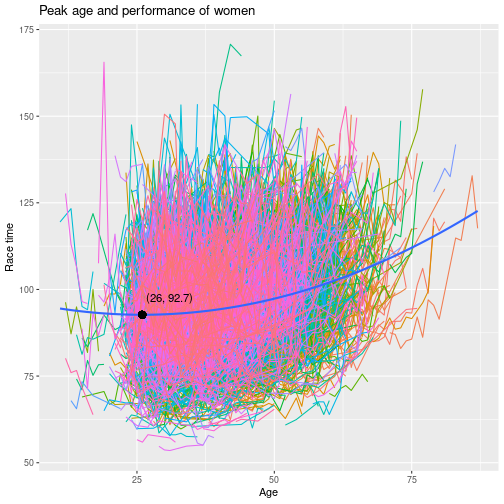
\includegraphics[width = \textwidth]
		{../figure/peak_plot2-2.png}
		\caption{}
		\label{peak-women}
	\end{subfigure}
	\caption{
		Estimation of peak performance of tracked runners.
	}
	\label{peak}
\end{figure}

% \begin{figure}
% 	\centering
% 	\includegraphics[width = 0.49\textwidth]
% 	{../figure/peak_plot2-1.png}
% 	\label{peak-men}
% 	\caption{I need a caption}
% \end{figure}

% \begin{figure}
% 	\centering
% 	\includegraphics[width = 0.49\textwidth]
% 	{../figure/peak_plot2-2.png}
% 	\label{peak-women}
% 	\caption{I need a caption}
% \end{figure}

According to Hawkins and Wiswell (2019), maximal oxygen uptake---the main
correlate of running speed---varied in an inverse U trend across a lifetime,
it is possible that running performance follows a quadratic model.
From the average of the data we collected between men and women
(see Figure \ref{peak}.)
% (models [7] and [8]),
we have determined the peak age is 26.5 years for men and 26 years for women.
On average, at these ages, the peak time of runners is between 77.1--77.9
minutes for men and 92.2-93.2 minutes for women (95\% confidence level).
% With this, we can see that men will generally have a faster peak than women.
% However, the rate at which age decreases their physical performance is much
% higher than women.
With this, we can see that men will generally have a faster peak than women. However, the rate at which age decreases their physical performance is much higher than women.
See Figure \ref{peak}.


\section*{Conclusions}

Using crossectional and panel analysis, this study found that age is a
strong predictor of physical performance.
Median runners need around 80-90 minutes to complete the 10-mile footrace.

On average women are slower than men by 26\%.
However, the rate of slowing down among women is certainly slightly lower
than that of men. Declining rates are different for different types of runners.
Average performers have the lowest declining rate in running speed.
The fastest runners have a higher average declining rate compared to the
average runner, while the slowest runners slow down significantly more than
the other groups.

Under the assumption that running time follows a U-shape trend across a
lifetime, peak performance ages for runners are predicted to be the mid-20s,
where the average running time of men is about 77.1--77.9 minutes and that of
women is about 92.2--93.2 minutes.

Limitations of this study are the generalizability of the result and the lack of relevant information that might bias the results. Because this is an observational study, without a well-representative dataset, the estimated effect of aging on physical activity can be only restricted to runners who are probably participating in the Cherry Blossom 10-mile run, with its own particular topographical characteristics and weather conditions in the DC’s springtime. Furthermore, without a carefully designed experiment or availability of relevant information (for example, training levels, lifestyle, etc), the estimated relationship can be upward or downward biased, depending on the relationship between the omitted factors and physical activity.

From this study, some further exploring questions can lead to a better understanding of the aging effect such as: How do women have a lower rate of decline in physical performance than men? Is the average peak age of women lower than men in any discipline of running or the observation is confined to the 10-miles marathon? What are the best strategies for training/exercises for runners of different age groups to maintain their long-term performance?

\section*{Recommendations}

This study and further investigation will benefit from more data collection efforts. Some useful background information such as pre-racing training levels or the number of running years should be collected for better estimation. Representativeness of data is also a potential issue since the race tends to attract more local people. Different geographical and environmental factors can play a role in runners’ performance. However, collecting all the historical information on the residency (location and duration) of runners can be a challenge with confidentiality barriers and people’s willingness to disclose/make up sensitive information. Therefore, if the race is advertised more widely and more approachable to other regions, the pool of participants can have better coverage of all geographical areas, the effect of which can be turned into noise rather than a systematic skewness to the East Coast runner population.

\begin{thebibliography}{9}

	\bibitem{HawkinsWiswell2003}
	Hawkins, S. A., \& Wiswell, R. A. (2003).
	Rate and Mechanism of Maximal Oxygen Consumption Decline with Aging:
	Implications for Exercise Training. Sports Medicine (Auckland), 33(12),
	877--888.
	\\
	\url{https://doi.org/10.2165/00007256-200333120-00002}


\end{thebibliography}


\appendix

\section{Appendix}

For the confidence levels used and inference to hold,
the noise should follow Normal distribution.
This is confirmed by the Q-Q plot of the estimated residuals,
provided in Figure \ref{qq}.

\begin{figure}[hb]
	\centering
	\includegraphics[width = 0.7\textwidth]
	{../figure/Image.png}
	\caption{
		Q-Q plot for estimated residuals.
	}
	\label{qq}
\end{figure}

\end{document}